%%%%%%%%%%%%%%%%%%%%%%%%%%%%%%%%
% SECTION :: IR in our project %
%%%%%%%%%%%%%%%%%%%%%%%%%%%%%%%%
\section{IR in our project}
%%%%%%%%%%%%%%%%%%%%%%%%%%%%%%%%%%%
% Frame Open :: IR in our project %
%%%%%%%%%%%%%%%%%%%%%%%%%%%%%%%%%%%
\frame{\frametitle{IR in our project}
\begin{itemize}
\item
Designing a good IR is more art than science.
\item
Specially true in our project where there's only
one source language (Poseidon) and
one target language (MIPS).
\item
In fact, do we even \textit{need} an IR in our project?
\textbf{Why not translate directly AST $\rightarrow$ MIPS}?
\item
For example, how should we \textit{really} translate \textit{32765+8}?
(remember that addition is done with 16 bits overflow).
\begin{itemize}
\item
Should we handle overflow in AST $\rightarrow$ IR phase?
\item
Or should we handle it in the IR $\rightarrow$ MIPS phase?
\end{itemize}
\end{itemize}
\begin{figure}[htbp]
\begin{center}
% Requires \usepackage{graphicx}
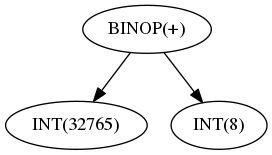
\includegraphics[width=4.0cm]{AST.png}\\
\label{Figure_Simple_Addition_Of_2_Integers_AST}
\end{center}
\end{figure}
%%%%%%%%%%%%%%%%%%%%%%%%%%%%%%%%%%%
% Frame Close :: Warm up examples %
%%%%%%%%%%%%%%%%%%%%%%%%%%%%%%%%%%%
}